\chapter{Firewall Avanzati}

Applicazioni come Telnet, SSH, rlogin \dots sono semplici da gestire con 
packet filtering, perché per loro natura implicano ruoli ben definiti: client 
e server; il pattern di scambio è un semplice request/reply.

Altre applicazioni possono avere protocolli più elaborati; quando lo 
scambio a livello di trasporto diventa più articolato, gestire il firewall 
diventa più complesso:
\begin{itemize}
    \item studiare molto bene i protocolli applicativi 
    \item verificare debolezze del filtraggio 
    \item essere consapevoli di cosa non si riesce a fare con il filtraggio 
\end{itemize}

\section{Packet Filtering Avanzati}

\subsection{SMTP (Simple Mail Transfer Protocol)}
Gestisce lo scambio di messaggi di posta elettronica:
\begin{itemize}
    \item la connessione tra i diversi server di posta avviene attraverso una connessione 
    TCP (porta 25)
    \item Ogni utente è identificato dall'indirizzo \textit{nomeutente@indirizzo\_server}
\end{itemize}

\noindent Il client a livello utente utilizza SMTP solo per inviare il messaggio al 
server mail, il quale poi lo invierà \textit{"davvero"}.

\subsubsection{I comandi}
I principali comandi SMTP:
\begin{itemize}
    \item \textbf{HELO}: identifica il client SMTP al server SMTP
    \item \textbf{EHLO}: possibile usare anche questo comando per identificarsi, se supportato dal server
    \item \textbf{MAIL FROM $<$indirizzo mittente$>$}: indica mailbox del mittente 
    \item \textbf{RCPT TO $<$indirizzo destinatario$>$}: mailbox destinatario; è possibile 
    indicare molteplici destinatari 
    \item \textbf{DATA}: indica al server che quanto digitato successivamente sono i dati del messaggio di posta
    \item \textbf{RSET}: annulla i comandi precedentemente inviati nella sessione corrente 
    \item \textbf{VRFY $<$stringa$>$}: chiede al server se la stringa rappresenta un nome utente, ed in tal 
    caso visualizza il suo indirizzo 
    \item \textbf{HELP}: visualizza i comandi disponibili sul server 
    \item \textbf{NOOP}: non esegue alcuna operazione, restituisce un messaggio 250 (OK) se il server risponde 
    \item \textbf{QUIT}: termina la sessione corrente
\end{itemize}

\subsubsection{Le fasi}
Una sessione SMTP attraversa almeno sei fasi:
\begin{enumerate}
    \item Il client SMTP contatta il server sulla porta 25; se è in ascolto e 
    la connessione è accettata risponde con un messaggio 220 (\textit{Ready})
    \item Il client chiede di stabilire la connessione inviando il comando HELO seguito 
    dal FQDN (Fully Qualified Domain Name); se il server accetta risponde con 250 (OK)
    \item Il client indica il proprio indirizzo tramite il comando MAIL FROM; il server risponde 250 (OK)
    \item Il client indica i destinatari tramite RCPT TO; il server risponde 250 (OK) per ogni destinatario accettato 
    \item Il client comunica l'intenzione di scrivere il corpo del messaggio con DATA
    \item Completato il messaggio il server memorizza la mail; è possibile scrivere un nuovo messaggio 
    oppure inviare il comando QUIT, dopo il quale il server invia i messaggi e risponde con Closing (221); la 
    connessione TCP viene terminata
\end{enumerate}

\subsubsection{I codici di risposta}
Il server risponde ad ogni comando con un codice di tre cifre che ha la 
seguente interpretazione:
\begin{itemize}
    \item 1xx: messaggio informativo
    \item 2xx: comando eseguito e terminato con successo 
    \item 3xx: comando eseguito e terminato con successo che richiede di essere 
    seguito da altri comandi 
    \item 4xx: errore temporaneo nell'esecuzione del comando, ma il dialogo non è compromesso 
    \item 5xx: errore grave, il dialogo è compromesso e dovrà essere ripreso dall'inizio
\end{itemize}

\subsubsection{Protezione}
\begin{itemize}
    \item Protezione anti-spam minimale
    \begin{itemize}
        \item verifica del dominio del mittente 
        \item login obbligatorio
        
        $\rightarrow$ fatto per evitare \textbf{\textit{open relay}}, ovvero la capacità di mandare posta 
        senza essere autenticato 
    \end{itemize}
    \item Si aggiunge la criptazione al servizio di posta (con SSL/TLS); così viene criptata 
    il \textit{canale} ma non il messaggio, quindi un server intermediario può leggere 

    $\rightarrow$ se voglio criptare anche il messaggio si usa un altro protocollo (PGP)
\end{itemize}

\subsubsection{Packet Filtering}
\begin{itemize}
    \item \textbf{Politica:} nella rete aziendale un solo server SMTP è autorizzato 
    a gestire la posta elettronica con l'esterno 
    
    $\rightarrow$ bisogna gestire due connessioni TCP:
    \begin{itemize}
        \item Ricevere posta elettronica: altri mail server si connettono al mail server aziendale agendo da client 
        \item Inviare posta elettronica: il mail server aziendale si connette ad altri mail server agendo da client
    \end{itemize}
\end{itemize}

\begin{figure}[H]
    \centering
    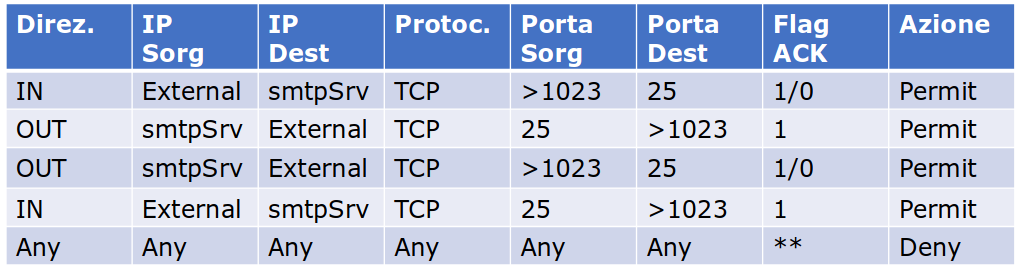
\includegraphics[width=1\linewidth]{chapters/12/images/smtp.png}
\end{figure}

\subsection{FTP (File Transfer Protocol)}
FTP è il protocollo generalmente usato per trasferire dati tra due host, con l'obiettivo 
di farlo in maniera efficiente ed affidabile; per questo motivo si basa su TCP (porta 21).

\noindent FTP utilizza due processi distinti:
\begin{itemize}
    \item \textit{Protocol Interpreter} (PI) attraverso cui il client invia comandi e riceve le risposte del server 
    \item \textit{Data Transfer Process} (DTP) attraverso cui il client ed il server si scambiano dati;
    può essere di due tipi:
    \begin{itemize}
        \item Attivo: il client contatta il server il quale da inizio alla connessione 
        \item Passivo: è prerorgativa del client anche dare il via alla connessione
    \end{itemize}
\end{itemize}

\subsubsection{Le fasi}
\begin{enumerate}
    \item Il client contatta il server sulla porta 21 usando il PI
    \item Autenticazione del client 
    \item Trasferimento dati tramite DTP 
    \item Termine della sessione TCP 
\end{enumerate}

\subsubsection{Connessioni FTP}
Ci sono due connessioni TCP per ogni sessione FTP:
\begin{itemize}
    \item \textbf{Connessione di controllo:} usata dal client per inviare i comandi e 
    dal server per comunicare i codici di risposta; viene aperta dal client che si connette 
    al server sulla porta TCP 21 
    \item \textbf{Connessione dati:} usata per il trasferimento dei file, viene aperta 
    dal server sulla porta 20
\end{itemize} 

\noindent La connessione dati viene aperta dal server verso il client:
\begin{center}
    \texttt{ftpServer:20} $\rightarrow$ \texttt{ftpClient:XXXX}
\end{center}

\noindent dove XXXX è la porta definita dinamicamente dal client.

\noindent $\rightarrow$ Non è possibile applicare la solita politica di gestione, dato che 
la connessione da esterno ad interno è obbligata ma non sappiamo a priori la porta.

\noindent Rischio:
\begin{center}
    \texttt{Intusore:20} $\rightarrow$ \texttt{Vittima:XXXX}
\end{center}

\noindent Le porte $>$1023 sono usate da servizi molto diffusi e da trojan.

\begin{figure}[H]
    \centering
    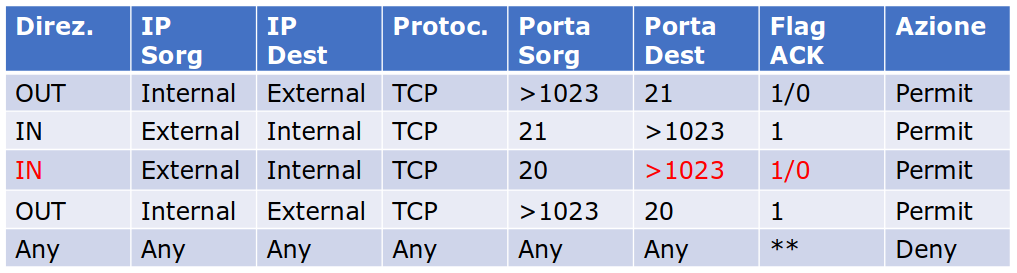
\includegraphics[width=1\linewidth]{chapters/12/images/ftp1.png}
\end{figure}

\noindent Dovrei usare un packet filtering che si ricordi delle connessioni.
\subsubsection{Soluzione}
La connessione dati viene aperta dal client verso il server (DTP passivo).

\begin{center}
    \texttt{ftpClient:YYYY} $\rightarrow$ \texttt{ftpServer:XXXX}
\end{center}

La politica di gestione \textit{connessioni solo da interno ad esterno} torna 
ad essere applicabile. Ora tutti gli FTP supportano la modalità passiva di default.

\begin{figure}[H]
    \centering
    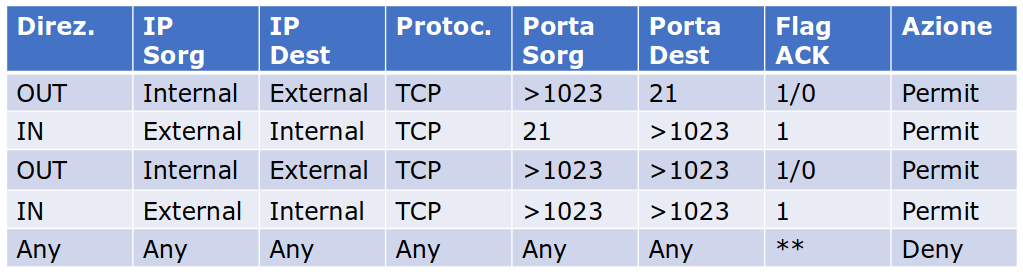
\includegraphics[width=1\linewidth]{chapters/12/images/ftp2.png}
\end{figure}

\subsection{Attacco RPC}
Remote Call Procedure è un protocollo che può essere utilizzato 
da un'applicazione per richiedere un serivizio a un programma residente su un 
altro computer in rete. 
\noindent È stata riscontrata una vulnerabilità che potrebbe portare all'esecuzione 
di codice non autorizzato.

\noindent A livello di firewall il problema è che non si conosce a priori la
porta che il server RPC assegnerà al servizio. Rischio:
\begin{center}
    \texttt{Intrusore:YYYY} $\rightarrow$ \texttt{ServerRPC-Vittima:XXXX}
\end{center}

\section{New Generation Packet Filtering}

Lo svantaggio principale dell'approccio SPF risiede nell'\textbf{array di porte 
che devono essere lasciate aperte} per tutto il tempo per permettere il 
traffico desiderato.

\subsubsection{Dynamic Packet Filter}

\noindent Per superare questo problema sono stati sviluppati dei \textbf{Dynamic Packet Filter},
che aprono e chiudono le porte sul firewall in base alle info dell'header dei 
pacchetti che transitano attraverso di essi; una volta che una serie di pacchetti 
ha transitato attraverso la porta, il firewall richiude la porta.

\subsubsection{Stateful Packet Filter}
È una evoluzione del dynamic ma \textit{state-aware}:
\begin{itemize}
    \item prende informazioni dai livelli superiori (trasporto e/o applicativo) per cercare di adattare 
    di conseguenza le regole di filtraggio 
    \item distingue le nuove connessioni da quelle già apert, tenendo traccia delle sessioni
\end{itemize}

\subsection{Vantaggi e Svantaggi del Dynamic Packet Filter}
\begin{itemize}
    \item \textbf{\textcolor{darkgreen}{Vantaggi:}}
    \begin{itemize}
        \item le porte sono aperte solo temporaneamente sul perimetro della rete 
        \item supporta quasi tutti i servizi 
        \item molti attacchi che funzionano su SPF sono difficili o impossibili da replicare 
        su DPF
    \end{itemize}
    \item \textbf{\textcolor{red}{Svantaggi:}}
    \begin{itemize}
        \item permettono connessioni IP dirette verso gli host interni della rete
        \item non garantiscono alcuna autenticazione
        \item soggetto ad attacchi che mirano alla saturazione della tabella  
    \end{itemize}
\end{itemize}

\subsection{Connessioni TCP - stateful firewall}
\begin{itemize}
    \item Alla ricezioni di un SYN $\rightarrow$ verifica dell'ACL
    \begin{itemize}
        \item connessione non autorizzata $\rightarrow$ deny 
        \item connessione autorizzata $\rightarrow$ accept e scrittura di una entry nella connection table 
    \end{itemize}
    \item Ricezione di pacchetti successivi $\rightarrow$ verifica della connection table
\end{itemize}

\noindent $\rightarrow$ è necessario definire solo le regole relative all'apertura delle 
connessioni TCP (pacchetto SYN)

\subsection{UDP - stateful firewall}
UDP non ha uno stato della connessione per definizione; viene impostato dunque un \textbf{timeout}
verificando anche chi ha impostato la connessione per primo.
\noindent Molti sistemi stateful hanno la possibilità di fare filtraggio applicativo:
\begin{itemize}
    \item comporta che il firewall faccia il parsing del pacchetto e conosca i protocolli 
    \item tutto ciò a scapito delle performance
\end{itemize}

\subsection{Deep Packet Inspection}
Il controllo non viene fatto solo sul protocollo ma anche sul pattern di comunicazione usato. Ad 
esempio, le richieste che rispettano il protocollo ma sono tipicamente usate per un attacco vengono respinte.
\begin{itemize}
    \item offre una protezione migliore
    \item definizione più semplice della politica 
    \item impatta pesantemente sulle prestazioni
\end{itemize}


\section{Proxy}
Una tecnica di proxy serve per introdurre un componente che media le comunicazioni 
tra altri due componenti; \textbf{disaccoppia la comunicazione tra due componenti 
rendendola indiretta}.

\begin{figure}[H]
    \centering
    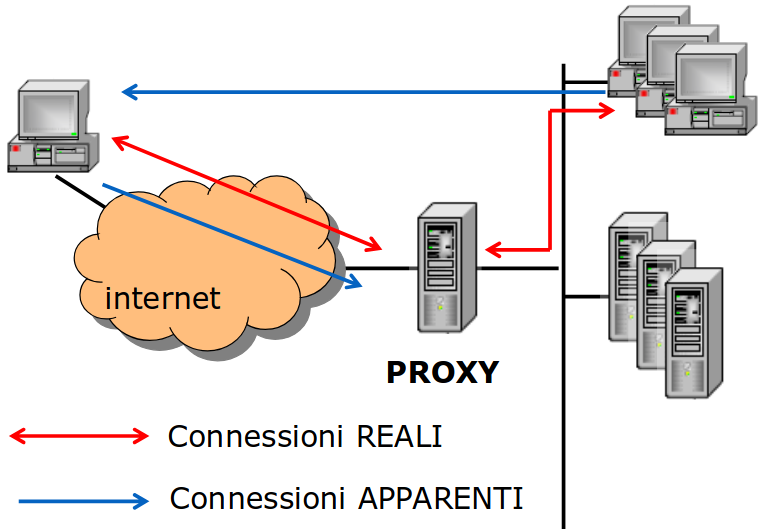
\includegraphics[width=0.8\linewidth]{chapters/12/images/proxy.png}
\end{figure}

\subsection{Reverse proxy}
Garantiscono l'accesso da utenti esterni a risorse interne; ad esempio, 
un server HTTP che fa solo da front-end e poi passa le richieste 
al vero server.

\begin{figure}[H]
    \centering
    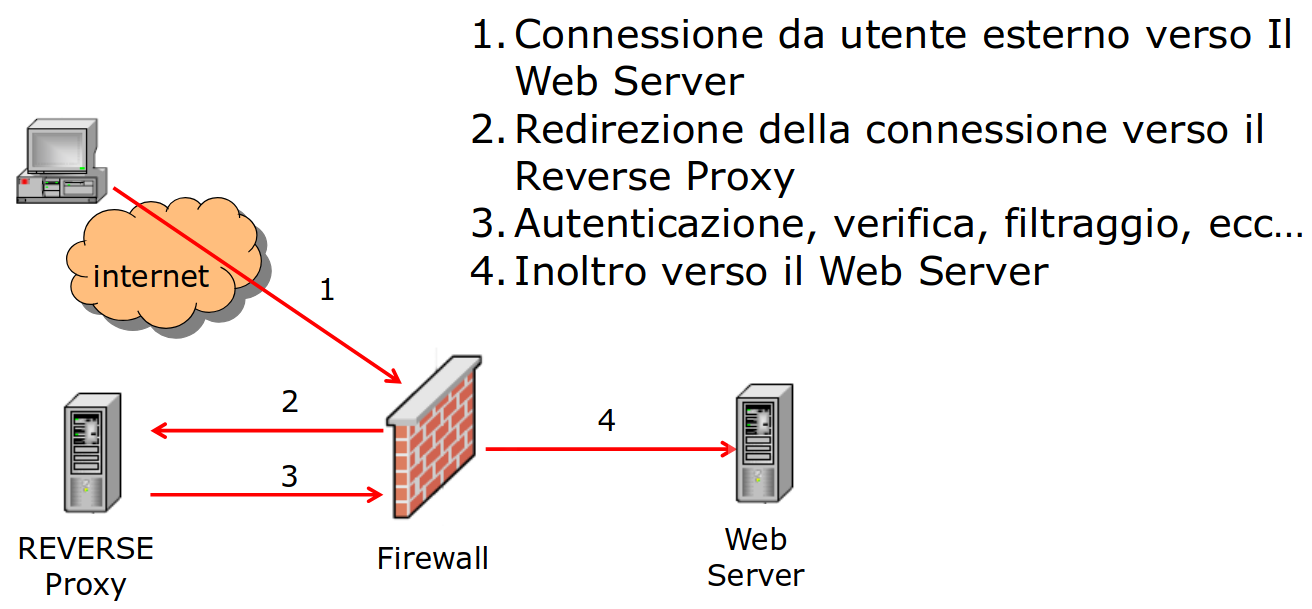
\includegraphics[width=0.9\linewidth]{chapters/12/images/reverse-proxy.png}
\end{figure}

\subsection{Proxy firewall: application-level gateway}
È composto da una serie di proxy che esaminano il contenuto dei pacchetti 
a livello applicativo.
\begin{itemize}
    \item Implementa funzioni di autenticazione 
    \item Può mascherare/rinumerare gli indirizzi IP interni 
    \item Si richiede uno specifico proxy per ogni applicazione
\end{itemize}

\noindent $\rightarrow$ ne segue che:
\begin{itemize}
    \item \textbf{\textcolor{darkgreen}{Vantaggi:}}
    \begin{itemize}
        \item non permette connessioni dirette tra esterno ed interno 
        \item supporta autenticazione
        \item analizza i comandi a livello applicativo 
        \item mantiene un log del traffico 
        \item analisi migliore del traffico applicativo rispetto a firewall stateful 
    \end{itemize}
    \item \textcolor{red}{\textbf{Svantaggi:}}
    \begin{itemize}
        \item introduce latenza, peggiora le performance
        \item limitazioni in termini di supporto
        \item vulnerabilità del firewall maggiormente esposte
    \end{itemize}
\end{itemize}

\subsection{Proxy firewall: circuit-level gateway}
È un proxy \textit{"application-aware"}; crea un circuito tra client e server 
a livello di trasporto:
\begin{itemize}
    \item non ha nessuna comprensione dei dati in transito 
    \item guarda gli header
\end{itemize}

\noindent Le fasi sono:
\begin{enumerate}
    \item il client crea una connessione TCP verso il circuit-level gateway e chiede 
    di stabilirne un'altra verso il verso server target 
    \item il gateway può controllare l'IP e autorizzare il client 
    \item il gateway contatta il server target e rigira il traffico e le richieste del client
\end{enumerate}

\noindent $\rightarrow$ ne segue che:
\begin{itemize}
    \item \textcolor{darkgreen}{\textbf{Vantaggi:}}
    \begin{itemize}
        \item rompe il modello client/server per la durata della connessione 
        \begin{itemize}
            \item server più protetti 
            \item isola da attacchi che riguardano handshake TCP 
            \item isola da attacchi che riguardano frammentazione IP 
            \item può autenticare il client 
        \end{itemize}
    \end{itemize}
    \item \textcolor{red}{\textbf{Svantaggi:}}
    \begin{itemize}
        \item molte limitazioni proprie del packet filter rimangono
    \end{itemize}
\end{itemize}

\subsection{Bastion host}
Il bastion host è un host critico per la sicurezza e costituisce la piattaforma per i gateway 
a livello di applicazione e circuito; si pone dunque tra la connessione pubblica 
e quella privata.

\noindent Le caratteristiche che dovrebbe avere sono:
\begin{itemize}
    \item un sistema operativo sicuro 
    \item avere solo i servizi proxy strettamente necessari 
    \item servizi di autenticazione 
    \item sistemi di logging e auditing
\end{itemize}

\subsection{Proxy firewall: conclusioni}
\begin{itemize}
    \item può essere utilizzato per analizzare i dati delle applicazioni perché
    opera a livello applicativo 
    \item performance potenzialmente molto critiche 
    \item analisi migliore del traffico applicativo rispetto ad uno stateful firewall
\end{itemize}

\section{Architetture e scenari}
\subsection{Screened host firewall}

\subsubsection{Single-homed}

\begin{figure}[H]
    \centering
    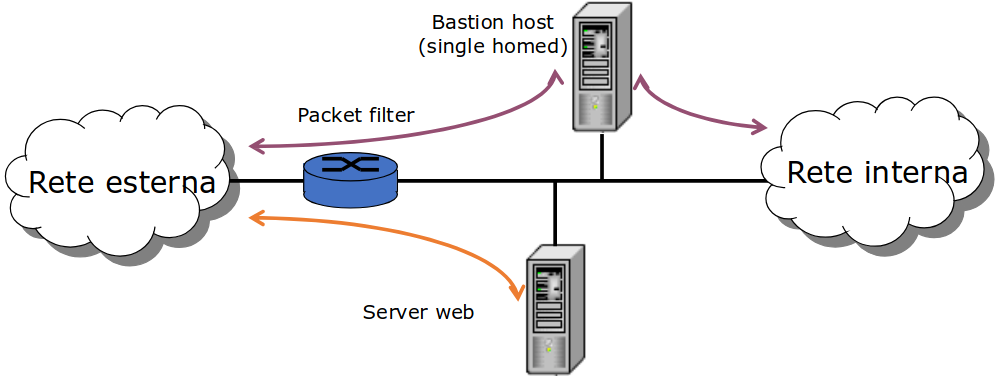
\includegraphics[width=1\linewidth]{chapters/12/images/single-homed.png}
\end{figure}

\begin{itemize}
    \item il packet filter fa passare i pacchetti provenienti dall'esterno e 
    diretti al bastion host (agisce da proxy)
    \item il packet filter può far passare i pacchetti provenienti dall'esterno e 
    diretti ad un server che non ha un livello di sicurezza elevato (es. server web)
    \item il packet filter fa passare i pacchetti provenienti dal bastion host e diretti verso l'esterno
    
    \item $\rightarrow$ il traffico viene analizzato due volte; se il packet filter viene compromesso 
    il bastion host sarebbe a difesa
\end{itemize}

\subsubsection{Dual-homed}

\begin{figure}[H]
    \centering
    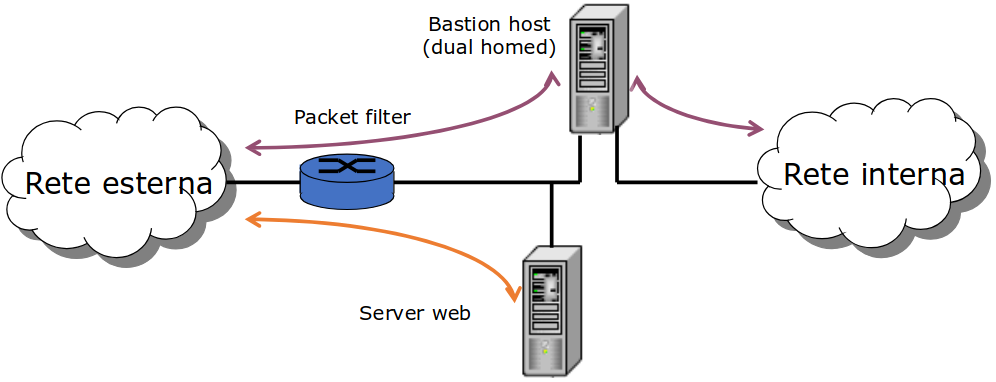
\includegraphics[width=1\linewidth]{chapters/12/images/dual-homed.png}
\end{figure}

\noindent Previene i problemi causati dalla compromissione del packet filter 
perché un pacchetto deve "fisicamente" attraversare il bastion host

\subsection{Screened subnet firewall}

\begin{figure}[H]
    \centering
    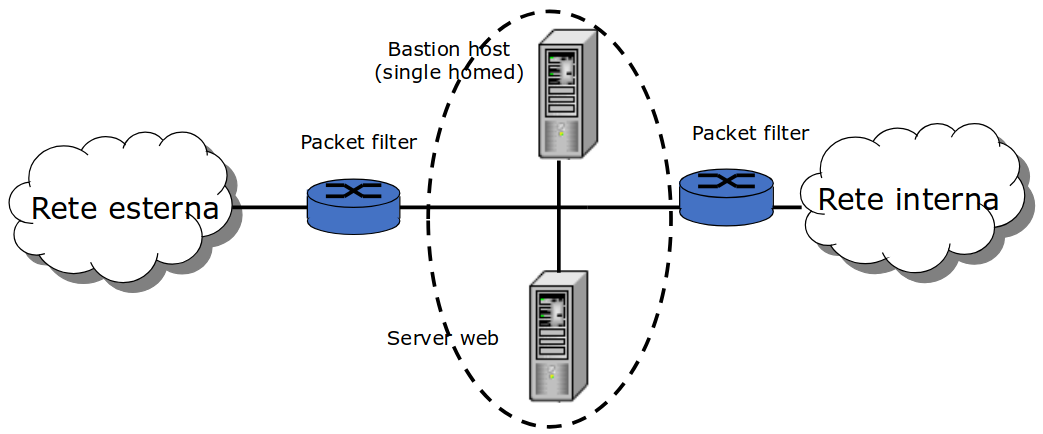
\includegraphics[width=1\linewidth]{chapters/12/images/subnet-firewall.png}
\end{figure}

È l'architettura più sicura tra quelle mostrate; la DMZ è accessibile 
sia dalla rete interna che esterna, ma il traffico deve obbligatoriamente 
passare per i packet filter.

\subsection{FTP bounce attack}
Il comando \texttt{PORT} di FTP ha la seguente sintassi:
\begin{center}
    \texttt{PORT h1, h2, h3, h4, p1, p2} dove:
    \begin{itemize}
        \item \texttt{h1, h2, h3, h4} rapprsentano gli ottetti dell'IP del server FTP 
        \item $(256 \cdot p1 + p2)$ restituisce la porta sulla quale il client riceverà al connessione dal server
    \end{itemize}
\end{center}

\noindent Ad esempio, \texttt{PORT 159, 149, 10, 5, 4 ,1}

$\rightarrow$ IP: 159.149.10.5

$\rightarrow$ Porta: 1025

\subsubsection{Attacco}
\noindent Lo scenario dell'attacco è il seguente:
\begin{itemize}
    \item sono ammesse connessioni dall'esterno verso l'FTP server 
    \item il Telnet server è accessibile solo dall'interno
\end{itemize}

\begin{figure}[H]
    \centering
    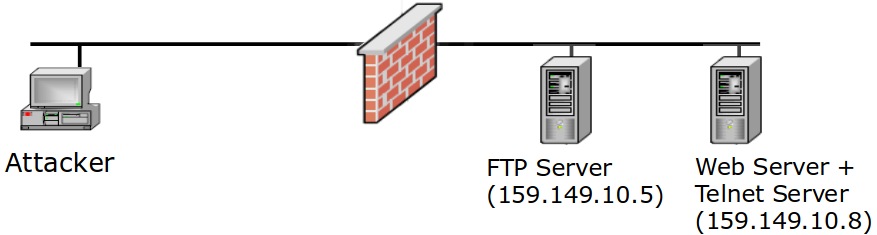
\includegraphics[width=1\linewidth]{chapters/12/images/ftp-bounce.png}
\end{figure}


\begin{enumerate}
    \item l'attaccante si connette all'FTP server, mandando il comando:
    \begin{center}
        \texttt{PORT 159, 149, 10, 8, 0, 23}
    \end{center}
    con il quale si impone all'FTP server che il successivo trasferimento di file dovrà
    essere fatto verso il Telnet server (porta TCP)
    \item invia il comando \texttt{RETR}; questo causa l'apertura di una connessione 
    da FTP server a Telnet server 
\end{enumerate}

$\rightarrow$ la protezione perimetrale è stata \textit{bypassata}, è possibile 
far eseguire comandi

\noindent Questo attacco è risolvibile con uno \textit{stateful firewall}, o con 
un FTP proxy che potrebbe riconoscere l'uso improprio del protocollo (in realtà è stato 
risolto con un aggiornamento a FTP).

\subsection{\textit{Best practices}}
\begin{itemize}
    \item usare un proxy per rompere fisicamente il percorso di rete 
    \item usare uno stateful packet filter, più resistente di uno stateless 
    \item disabilitare tutte le porte non strettamente necessarie (default deny)
    \item rendere sicuro il sistema operativo usato 
\end{itemize}

\section{Netfilter e IPTables}
Netfilter è il componente del kernel Linux che permette l'intercettazione e 
la manipolazione dei pacchetti. Implementa funzionalità avanzate come filtraggio 
stateful del traffico di rete.

\subsubsection{Funzionamento}

\noindent Il funzionamento di Netfilter è incentrato sull'utilizzo di tabelle, 
implementate a livello kernel. Ogni tabella contiene delle \textit{chain}, che 
sono delle ACL e contengono a loro volta delle \textit{rules}; ogni regola è divisa in 
due parti:
\begin{itemize}
    \item Filtro: proprietà che un pacchetto deve avere affinché la regola sia valida
    \item Target: azione da compiere nel caso il pacchetto corrisponda alle proprietà impostate 
    nel filtro
\end{itemize}

\subsubsection{Tabelle}

\noindent Netfilter ha quattro tipi di tabelle:
\begin{itemize}
    \item \textbf{filter:} tabella delle regole di filtraggio dei pacchetti; permette di scegliere 
    quali bloccare e quali far passare. Ha tre chain di base:
    \begin{itemize}
        \item \textit{Input:} tutti i pacchetti in arrivo destinati al sistema passano per questa catena 
        \item \textit{Forward:} tutti i pacchetti in arrivo (non generati dal sistema stesso) destinati ad un altro sistema passano per questa catena (es. un router)
        \item \textit{Output:} tutti i pacchetti generati dal sistema passano per questa catena
    \end{itemize}
    \item \textbf{nat:} tabella delle regole di traduzione degli indirizzi; per protocolli orientati alla sessione, solo 
    il primo pacchetto passa per questa tabella, gli altri appartenenti alla stessa sessione seguiranno la stessa decisione.
    
    \noindent Ha tre chain di base:
    \begin{itemize}
        \item \textit{Prerouting:} passano i pacchetti in entrata, prima che venga presa la 
        decisione di instradamento 
        \item \textit{Postrouting:} passano i pacchetti in uscita, dopo che è stata fatta la decisione 
        di instradamento
        \item \textit{Output:} permette la conversione degli indirizzi pubblici dei pacchetti in entrata sulla rete locale ai rispettivi indirizzi privati (DNAT) 
    \end{itemize}
    \item \textbf{mangle:} permette di fare modifiche alle opzioni dei pacchetti e di applicare politiche avanzate. Ha le seguenti chain:
    \begin{itemize}
        \item \textit{Prerouting:} esamina tutti i pacchetti in entrata nel sistema, prima che venga consultata la tabella di routing 
        \item \textit{Input:} esamina tutti i pacchetti in entrata nel sistema destinati al sistema stesso 
        \item \textit{Forward:} esamina tutti i pacchetti in entrata ma destinati ad un altro sistema
        \item \textit{Output:} esamina tutti i pacchetti generati dal sistema 
        \item \textit{Postrouting:} esamina tutti i pacchetti, dopo che è stata fatta la decisione di routing e prima di inoltrare effettivamente il pacchetto al sistema destinatario
    \end{itemize}
    \textbf{raw:} permette di evitare il tracciamento della connessione, nel caso in cui 
    si voglia avere un filtraggio stateless. Ha due chain:
    \begin{itemize}
        \item \textit{Prerouting:} provenienti da qualsiasi interfaccia di rete 
        \item \textit{Output:} generato dal processo locale
    \end{itemize}
\end{itemize}

\subsubsection{Targets}
I targets sono le azioni da compiere su un pacchetto. Possono essere:
\begin{itemize}
    \item Una chain - per far gestire il pacchetto ad una catena specifica definita manualmente
    \item Uno dei target predefiniti:
    \begin{itemize}
        \item ACCEPT 
        \item DROP, REJECT 
        \item QUEUE 
        \item LOG 
        \item \dots
    \end{itemize}
    \item Un obiettivo definito da un'estensione
\end{itemize}


\subsection{IPTables}
IPTables è un tool per configurare Netfilter.

\medskip

\noindent \textit{si consiglia di guardare le slide per i 
comandi e gli esericizi riguardanti IPTables (M1\_UD2\_L5 / M1\_UD2\_L6)}




